\setAuthor{}
\setRound{lõppvoor}
\setYear{2020}
\setNumber{G 4}
\setDifficulty{4}
\setTopic{TODO}

\prob{Tasakaaluliikur}
\begin{wrapfigure}{r}{0.35\textwidth}
  \vspace{-5pt}
  \begin{center}
  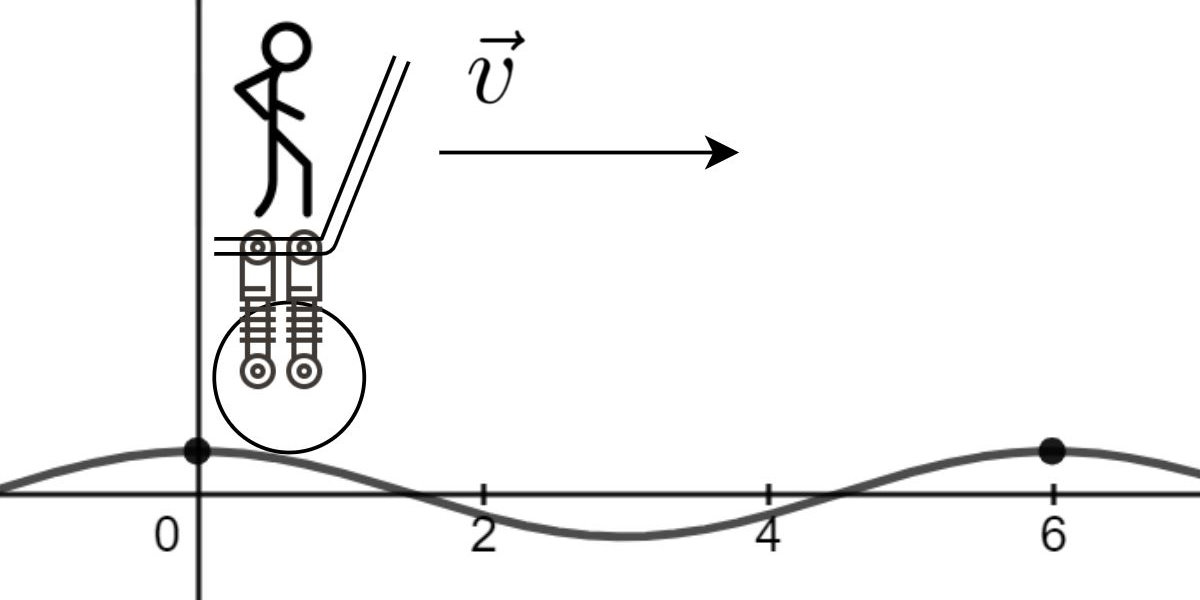
\includegraphics[scale=0.1]{2020-v3g-04-yl.png}
  \end{center}
  \vspace{-25pt}
\end{wrapfigure}
Hannes massiga $m = \SI{75}{\kilo\gram}$ sõidab tasakaaluliikuriga  konarlikul
teel ühtlase kiirusega $v$. Konarliku tee profiili saab külgvaates lähendada
koosinuslainele amplituudiga~$A = \SI{60}{\milli\meter}$ ja
perioodiga~$\Delta x = \SI{6}{\meter}$. Tasakaaluliikuril on amortiseerimissüsteem,
mis koosneb $n=2$ rööbiti ühendatud vedrust jäikusega $k = \SI{900}{\newton\per\meter}$.
Leidke kiirus~$v$, mille juures Hannes võngub enim ehk tekib resonants.
Tasakaaluliikuri kaal on tühine. Kiirus $v$ on kiirus, mida näitaks
tasakaaluliikuril olev GPS seade, mitte ratta keerlemisel põhinev odomeeter.

\emph{Vihje:} Kui keha kiirendus $a$ ja kaugus tasakaalupunktist $y$ on seotud
võrdusega $a=-\omega^2 y$, kus $\omega$ on positiivne konstant, siis võngub keha
perioodiga~$\frac{2\pi}{\omega}$.


\hint

\solu
Hannese liikumist saab vertikaalsuunas käsitleda vedrupendli võnkumisena. Vedrupendli perioodi valem on: $$T=2\pi \sqrt{\frac{m}{k}}$$ Kuna meie süsteemil on kaks vedru rööbiti, tuleb võngete perioodi valemit veidi muuta. Kahe kõrvuti oleva vedru jäikus on võrdne ühe vedruga, mille jäikus on eelnevate vedurude jäikuste summaga. Seega on meie süsteemi vertikaalsuunaliste võngete periood:
$$T = 2\pi \sqrt{\frac{m}{2k}}$$
Resonants tekib, kui koosinuslaine läbimise sagedus ühtib verikaalse vedrusüsteemi naturaalsagedusega. Seega peab Hannes $\Delta x = \SI{6}{m}$ võrra edasi liikuma sama ajaga, mil teeb masspendel ühe naturaalsagedusel võnke. Seega, resonantsi tekke kiirus:
$$v_\mathrm{resonants}=\frac{\Delta x}{T}=\frac{\Delta x}{2 \pi} \sqrt{\frac{2k}{m}} = \SI{4.678}{m s^{-1}} \approx \SI{4.7}{m s^{-1}}$$
\probend